\documentclass[uplatex, titlepage, fontsize=10pt, paper=a4paper]{jsarticle}
\usepackage[top=20truemm,bottom=20truemm,left=20truemm,right=20truemm]{geometry}
% 数式
\usepackage{amsmath,amsfonts}
\usepackage{bm}
% 画像
\usepackage[dvipdfmx]{graphicx}
\usepackage{wrapfig}

\numberwithin{equation}{section}

%\usepackage[subrefformat=parens]{subcaption}
\makeatletter

\def\@maketitle{
\begin{center}
{\Huge \@title }
\end{center}
\begin{center}
{\@author}
\end{center}
}

\makeatother

%\pagestyle{empty}

\title{
\vspace{-5cm}
--------------------------------------------------------------------------------------\\
\vspace{8mm}
{\Huge 光干渉計による光波スペクトル測定}\\
\vspace{6mm}
--------------------------------------------------------------------------------------}

\author{\Large
    \vspace{2mm}
    提出者\\
    \large
    \vspace{2mm}
    T200D507 齋藤瑚汰朗\\\\
    \Large
    \vspace{2mm}
    共同実験者\\
    \large
    \vspace{2mm}
    T200D053 小松美咲\\
    \large
    \vspace{2mm}
    T200D052 小堀祥汰\\
    \large
    \vspace{2mm}
    T200D050 小林雄馬\\
    \large
    T200D047 高 健智
    \vspace{5mm}
}

\date{\Large
    実験日(一日目) 2022年4月18日\\
    \Large
    \vspace{2mm}
    実験日(二日目) 2022年4月25日
}



\begin{document}

\maketitle

\newpage

\section{実験目的}
光通信の分野では、波長の異なる光に各々の情報を重ね合わせて、一本の光ファイバで同時に伝送する、いわゆる波長分割多重(WDM:Wavelength Dvision Multipleexing)光通信システムが多く採用されている。このWDM光通信システムは、多数の波長成分が含まれる多重化後の光信号の光スペクトルを高精度に測定する必要がある。この実験では、光干渉計を利用して光のスペクトルを測定し、フーリエ変換分光法の基礎を習得することが目的である。

\section{原理}

\begin{wrapfigure}{r}[10pt]{0.5\textwidth}
    \centering
    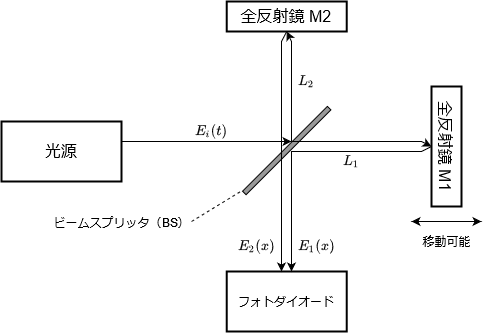
\includegraphics[width = 0.5\textwidth]{画像フォルダ/Interferometer.png}
    \caption{マイケルソン干渉計の構成}
    \label{Michelson_interferometer}
\end{wrapfigure}

光源から射出された光をビームスプリッタ(BS)を用いて二分する。二分したビームの一方は固定反射鏡2へ向かい、もう一方は移動反射鏡M1へ向かう。二分された光は、それぞれM1、M2によって反射して再びBSに戻って合成される。ここで入射光の電場の周波数$\nu$を式\ref{equation_E_i}で表すとする。($a(\nu)$:振幅、$t$:時間)

\begin{equation}
    E_{i}(t) = a(\nu)\exp(i2{\pi\nu}t)
    \label{equation_E_i}
\end{equation}

BSを透過・反射するさいに振幅にかかる係数をそれぞれ$t_{BS}$,$r_{BS}$とし、この瞬間に生じる位相変化をそれぞれ$\delta_{1}$,$\delta_{2}$とする。固定反射鏡M1・移動反射鏡M2から反射し、再びBSに戻ってきた光の電場は、式\ref{equation_E_M1}と式\ref{equation_E_M2}のように示すことができる。

\begin{equation}
    E_{1}(\nu, t) = t_{BS}a(\nu)\exp\left[i\left\{{2{\pi\nu}t-{\frac{2{\pi\nu}L_1}{c}}+\delta_1}\right\}\right] 
    \label{equation_E_M1}
\end{equation}

\begin{equation}
    E_{2}(\nu, t) = r_{BS}a(\nu)\exp\left[i\left\{{2{\pi\nu}t-{\frac{2{\pi\nu}L_2}{c}}+\delta_2}\right\}\right] 
    \label{equation_E_M2}
\end{equation}

$t_{BS}=r_{BS}=1/\sqrt{2}$の時、BSの反射と通過がそれぞれ一度だけ発生した事に留意して、フォトダイオードに入り込む合成光の電場は計算すると、

\begin{equation}
    \begin{split}
    E_{o}&=r_{BS}E_{1}(\nu,t)+t_{BS}E_{2}(\nu,t)\\
    &=\frac{1}{2}a(\nu)\left[\exp \left\{2\pi{i\nu}\left(t-\frac{L_1}{c}\right)+i\delta_1 \right\}+\exp \left\{2\pi{i\nu}\left(t-\frac{L_2}{c}\right)+i\delta_2 \right\} \right] 
    \label{equation_E_o}
    \end{split}
\end{equation}

となる。光強度は振幅の二乗に比例する。よって、合成波の電場の強度は式\ref{equation_E_strength}のように示すことができる。

\begin{equation}
    {\left\lvert E_{o}(\nu, t)\right\rvert} ^2 = \frac{1}{2}a^{2}(\nu)\left\{1+\cos\left(2\pi\nu\frac{L_{1}-L_{2}}{c}+\delta_{2}-\delta_{1}\right) \right\} 
    \label{equation_E_strength}
\end{equation}

従って、合成波を受光したフォトダイオードの出力は、${\left\lvert E_{o}\right(\nu,t)\rvert}^2$に比例した電流が発生し、反射鏡M1を移動させて、$L_{1}$を連続的に変化させる事で、$L_{1}$に対して交流的に変化する成分が光強度に含まれることになる。\\
ここで、$\tau=(L_{1}-L_{2}/c)$及び、$\delta=\delta_{2}-\delta_{1}$とすると、光強度は式\ref{equation_E_o_short}のように示せる。

\begin{equation}
    {\left\lvert E_{o}(\nu,t)\right\rvert}^2=\frac{1}{2}G(\nu)\cos(2\pi\nu\tau+\delta)
    \label{equation_E_o_short}
\end{equation}

\section{実験}

\subsection{注意事項}
実験を進める上で、注意すべき点について記述する。

\subsubsection{干渉計}


\subsubsection{光源}

\subsubsection{光ファイバーケーブル}


\section{実験結果}


\section{考察}

\subsection{マイケルソン干渉計における光出力強度}
He-Neレーザ光を用いた場合、周期的な信号が観測される。干渉計への入力が一定であることを考えると、エネルギー保存則によってフォトダイオードからの出力は一定でなければならない。しかし、実際にオシロスコープで観測した波形は周期的に変化している。フォトダイオードからの出力が最大でない場合、残りのエネルギーがどのような振る舞いをしたのかを考える。

\begin{wrapfigure}{r}[10pt]{0.5\textwidth}
    \centering
    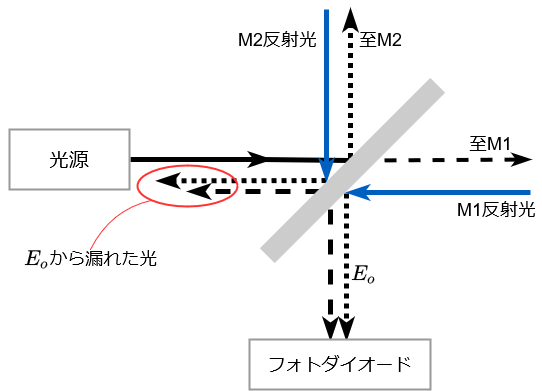
\includegraphics[width = 0.5\textwidth]{画像フォルダ/interference_detail.png}
    \caption{漏れる分の光}
    \label{interferometer_detail}
\end{wrapfigure}

\subsubsection{ビームスプリッタの役割}
式\ref{equation_E_o_short}によると、光強度は$L_{1}$によって周期的に変化することがわかる。そして、$\cos(2\pi\nu\tau+\delta)$が0となるときに、光強度も0となる。しかし、ここで注意するべき点は、\ref{equation_E_o_short}が示す光強度は、フォトダイオードに入り込む光の強度を示している事である。そこで、ビームスプリッタの作用について考える。ビームスプリッタは、光を二分する器具である。それを考慮すると、実際の光の道筋は図\ref{interferometer_detail}に示したような経路を辿っている事になる。この図の細かい点線が反射光、粗い点線が透過光を示している。図\ref{Michelson_interferometer}には、複雑さを回避するため表記を省略している。$L_{1}$を変化させると、M1の反射光とM2の反射光の一部は、BSに当たった際にフォトダイオード側に向かうことなく漏れ出ていく。これが、周期的に光強度が変化する原因である。\cite{wave_and_energy_conservation_law}

\subsection{ミラーの移動速度変動の影響の抑制}
反射鏡M2を波長オーダーの領域で等速で移動させることは難しい。一定の速度で移動しなくても$V(x)$の変化を正確にする方法を考える。

M1の移動とともに現れるビート信号の周期は、$x$の移動分にのみ依存し、レーザー波長の1/2だけ移動した時間がビート信号の周期に相当する。

\subsection{ASE光源の光スペクトルの類推}

\subsection{サイドロープの起源}

\subsection{FT-IRの特徴と今後}

\begin{thebibliography}{99}
    \bibitem{wave_and_energy_conservation_law}井上薫, and 山崎正之. "波の重ね合わせの原理とエネルギー保存則." 東海大学紀要工学部 45.2 (2005): l9-22.
\end{thebibliography}

\end{document}